\pdfoutput=1
\documentclass[pra,twocolumn,showpacs,amsmath,amssymb, aps, 10pt]{revtex4-1}

\usepackage{graphicx}%Include figure files
\usepackage{dcolumn}%Align table columns on decimal point
\usepackage{bm}% bold math
% \usepackage[page]{appendix}

\graphicspath{{../images/}}

%\nofiles

\begin{document}

\title{Project 2: Chaos in 1-D Scattering}


\author{John Russo}
\affiliation{Department of Physics and Astronomy, University
of Delaware, Newark, DE 19716-2570, USA}

\begin{abstract}
%TODO: Describe problem studied
%TODO: Describe how it was studied
%TODO: Describe major findings, conclusions
SWEET ABSTRACT GOES HERE
\end{abstract}

\pacs{45.40.Aa} %Translational kinematics


\maketitle

\section{Introduction} \label{sec:intro}

Classical systems that obey certain criteria can exhibit chaotic behavior, where
slight changes in initial conditions produce exponential divergence in behavior.
In other words, chaotic systems exhibit extreme sensitivity in initial
conditions. \cite{taylor}

In order to be chaotic, a system must exhibit:
\begin{enumerate}
  \item nonlinearity, \label{nonlinearity}
  \item dependence on more than three variables, and \label{dependence}
  \item sensitivity to initial conditions. \label{sensitivity}
\end{enumerate}

These conditions are necessary, but not sufficient to produce chaotic behavior.
A system can be chaotic for certain initial conditions but not others, as shown
in Section~\ref{sec:r9} below.

In this paper, behavior of a one-dimensional system of colliding balls is studied.
The balls are modelled as points which can elastically collide with each other
and with the floor. Dynamical equations of motion governing both the trajectories
of the balls and collisions between them are discussed
in Section~\ref{sec:methods}.

\begin{figure}[h]
  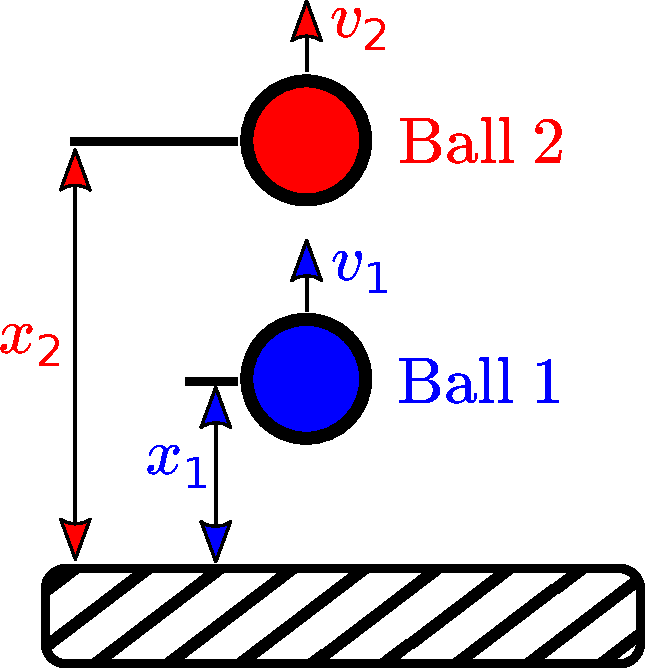
\includegraphics[width=.7\linewidth]{balls}
  \caption{Diagram of the one-dimensional system of balls simulated in this
  paper. The element at the bottom represents the floor upon which the bottom
  ball bounces.}
  \label{fig:balls}
\end{figure}

By varying parameters of the system such as the relative masses of the balls and
the initial positions and velocities of the balls, a wide range of dynamical
behavior can be exhibited. Of particular interest are the chaotic modes, where
minor variances in initial conditions cause exponential divergence in the positions
of the balls. The lens this system gives us into how varying initial
parameters it of particular interest for modelling and analysis to further
understand chaos.



\section{Methods} \label{sec:methods}

The system studied in this paper consists of two balls subject to gravity and
collisions with each other and the ground. Between collisions and bounces, each
ball obeys the one-dimensional kinematics equation

\begin{equation}
  x(t) = x_0 + v_0 t + \frac{1}{2} g t^2
  \label{eq:kinematics}
\end{equation}

where $x_0$ and $v_0$ refer to the position and velocity
of the ball after the previous collision or bounce, $x$ is the position of the ball,
$g$ is the acceleration due to gravity, and $t$ is the time since the previous
collision or bounce. %TODO: Repetitive phrasing here, also run-on of the ages

The normalization used is defined by
\begin{align}
x' &= \frac{mg}{E} x \\
v' &= \sqrt{\frac{m}{E}} v \\
t' &= \sqrt{\frac{mg^2}{E}} t \\
E &= \frac{1}{2} m_1 v_1^2 + \frac{1}{2} m_2 v_2^2 + m_1 g x_1 + m_2 g x_2
\label{eq:normalization}
\end{align}
where $E$ is the energy in non-normalized units.
Primes are used here to explicitly indicate normalized quantities.
In this normalization, $g$ is set to unity, and the equation of motion
Eq.~\ref{eq:kinematics} is written in terms of normalized variables as
\begin{equation}
x'(t) = x'_0 + v'_0 t' - \frac{1}{2} t'^2.
\label{eq:kinematics_normalized}
\end{equation}

Bounces and collisions are both characterized by elastic collisions in which
the total energy is conserved.

\subsubsection{Trajectory analysis algorithm}

The algorithm used to numerically evaluate the system follows a two-fold approach
to exactly solve for the positions of the balls at any time.

First, the positions, velocities, and times of each event are
computed sequentially, where event refers to either a collision between the two
balls or ball 1 bouncing off the ground.
Beginning with the initial conditions, the times for each
ball to reach the ground are computed. If the second ball would reach the ground
before the first, then a collision must occur before the first ball reaches the
ground. The time of this collision is determined by setting the equations of
motion for each ball, given by Eq.~\ref{eq:kinematics_normalized}, equal to each
other and solving for $t$.

If the event is a collision, then the velocities of the balls are updated according
to the equations for elastic collisions. For balls $1$ and $2$, these are

\begin{align}
  v_{1,f} &= \frac{m_1-m_2}{m_1+m_2}v_{1,i} + \frac{2 m_2}{m_1+m_2}v_{2,i} \\
  v_{2,f} &= \frac{2 m_1}{m_1+m_2}v_{1,i} - \frac{m_1-m_2}{m_1+m_2}v_{2,i}
\end{align}

where the subscript $i$ indicates the velocity immediately before the collision,
and the subscript $f$ indicates the velocity immediately after.

Bounces can only happen for ball 1. Ball 2 cannot hit the floor, since it would
collide with ball 1 first. If the event is a bounce, then the velocity of ball 1
is inverted so the ball is now travelling up. %TODO: Mention absolute value?

This algorithm continues until the first event outside of the desired maximum
time is detected.

In this way, the phase space coordinates and times of each event are calculated.
This is sufficient to plot Poincare sections, shown for ball 2 in
Section~\ref{sec:results}.

The second stage of the algorithm involves calculating the trajectories of each
ball. This is necessary both for plotting the spatial trajectories, and for
calculating autocorrelations.

To calculate autocorrelations, it is necessary %TODO: Is this true?
for the phase space coordinates of each ball to be determined evenly spaced in time.

Recall that between each event, the motion of each ball is given by
Eq.~\ref{eq:kinematics_normalized}. So, the motion is completely determined by
the phase space coordinates of the ball at the previous event, and the time
since that event.

A list of evenly-spaced timesteps at which the trajectories will be sampled at
is generated. For each interval between events, a function of the form
Eq.~\ref{eq:kinematics_normalized} is created, with the initial conditions $x'_0$
and $v'_0$ determined by the phase space coordinates of the previous event, along
with the start and end time of the interval.

Each timestep is iterated over, invoking the appropriate function for the
interval it falls in to evaluate the positions and velocities of the balls.

Further details on optimizations done to this algorithm are available
in Appendix~\ref{appendix:traj}.


\subsubsection{Autocorrelation}

Autocorrelations $a(\tau)$ were calculated for lag $\tau$ according to
\begin{equation}
  a(\tau) = \frac{1}{N-\tau} \sum_{i=1}^{N-\tau}
  \left(f_i - \bar f \right)
  \left(f_{i+\tau} - \bar f \right)
  \label{eq:acorr}
\end{equation}
where $N$ indicates the total number of datapoints, $f_i$ is the set of discrete
positions, and $\bar f$ is the mean of $f$.

Since the implementation of this provided acceptable runtimes even over datasets
on the order of hundreds of thousands of elements, no subsampling was performed.


%TODO: Include a section on how Lyapunov exponents were calculated.
% \subsubsection{Lyapunov Exponent}
%
% Lyapunov exponents



% TODO: Give numerical parameters like timestep, total time. Explain why Poincare
%   sections are run for longer time.



\section{Results} \label{sec:results}
% Each section should include initial conditions, or put in method
% Discuss physics
% Figures should support results, not the other way around

% Maybe reorganize this into nonchaotic -> partially -> chaotic.


%%%%%%%%%%%%%%%%%%%%%%%%%%% m2 = 0.5 m1 %%%%%%%%%%%%%%%%%%%%%%%%%%%%%%
\subsection{$m2 = 0.5 m1$}
% TODO: Plots of x1 and x2 vs t for m2 = 0.5 * m1, given initial conditions
\begin{figure}
  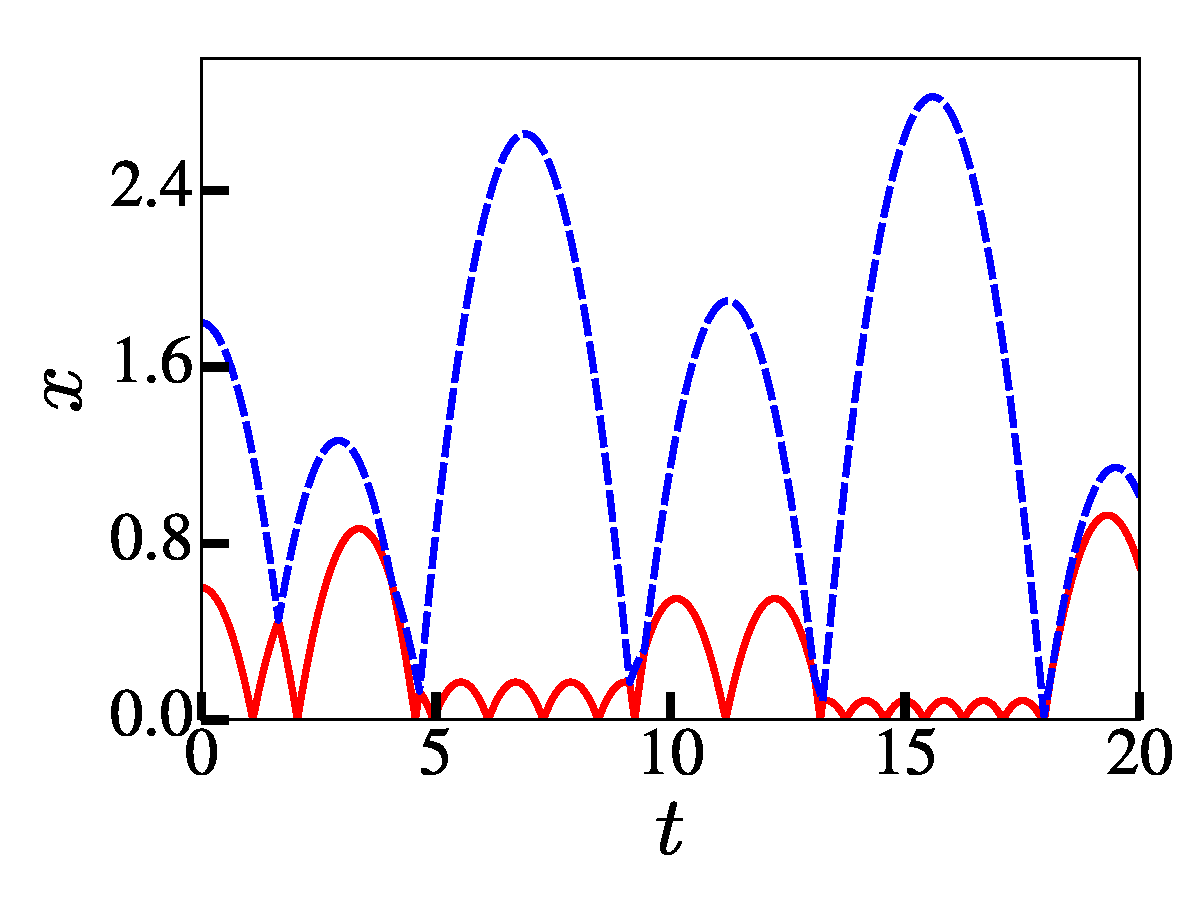
\includegraphics[width=0.8\linewidth]{r2_0_traj}
  \caption{Trajectories for two balls}
  \label{fig:0.5-traj}
\end{figure}

% TODO: Poincare section
\begin{figure}
  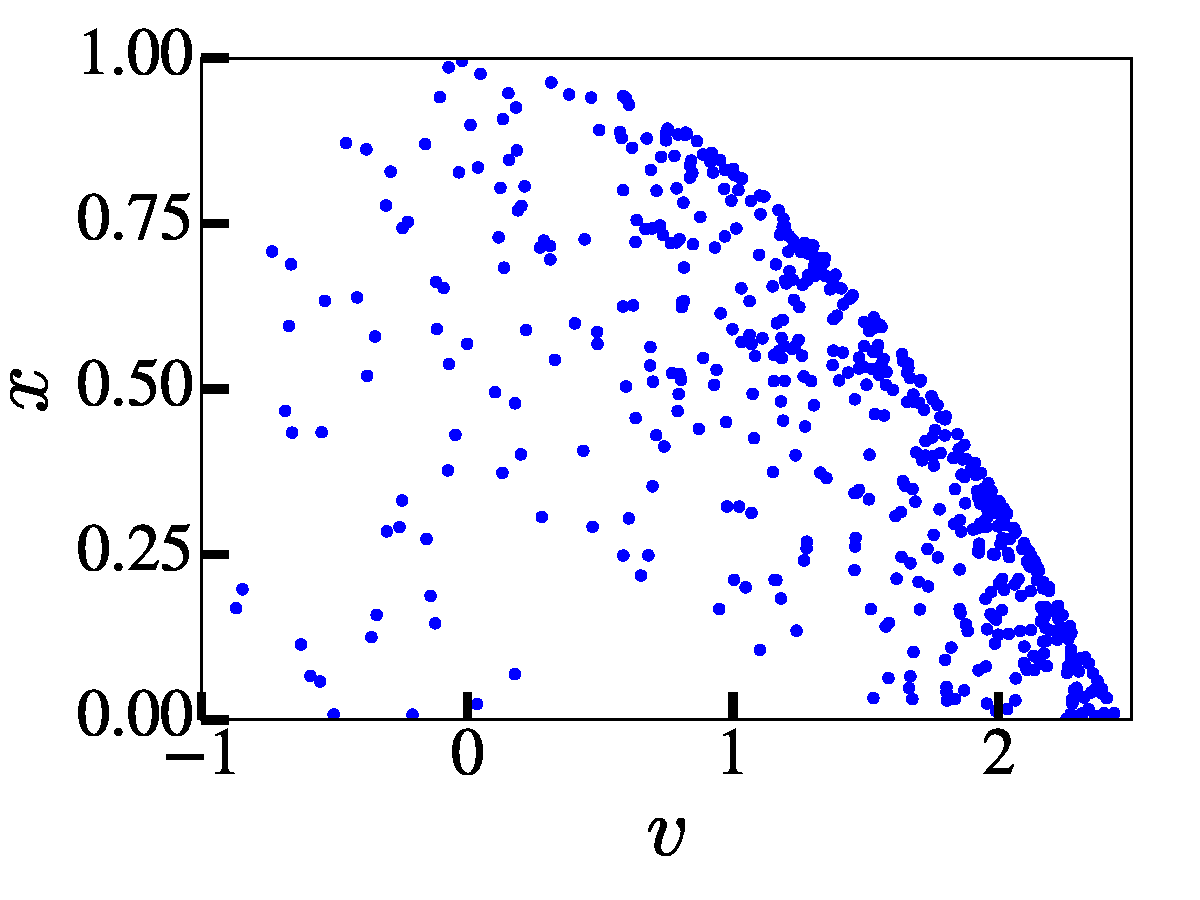
\includegraphics[width=0.8\linewidth]{r2_0_poincare}
  \caption{Poincare section for ball 2}
  \label{fig:0.5-poincare}
\end{figure}

% TODO: Autocorrelation function
\begin{figure}
  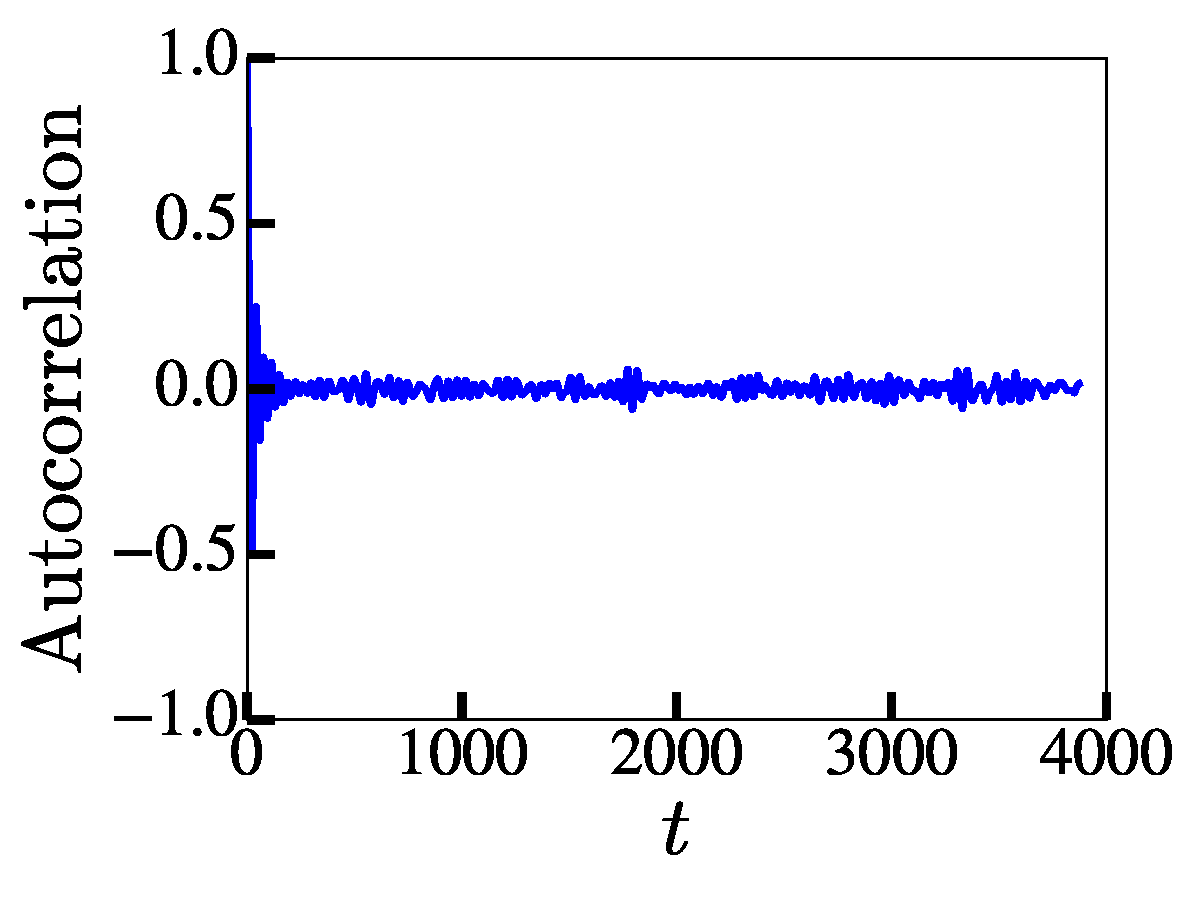
\includegraphics[width=0.8\linewidth]{r2_0_acorr}
  \caption{Trajectories for two balls}
  \label{fig:0.5-acorr}
\end{figure}

% TODO: Comment on which are chaotic




%%%%%%%%%%%%%%%%%%%%%%%%%%% m2 = m1 %%%%%%%%%%%%%%%%%%%%%%%%%%%%%%
\subsection{$m2 = m1$}
% TODO: Plots of x1 and x2 vs t for m2 = m1, given initial conditions
\begin{figure}
  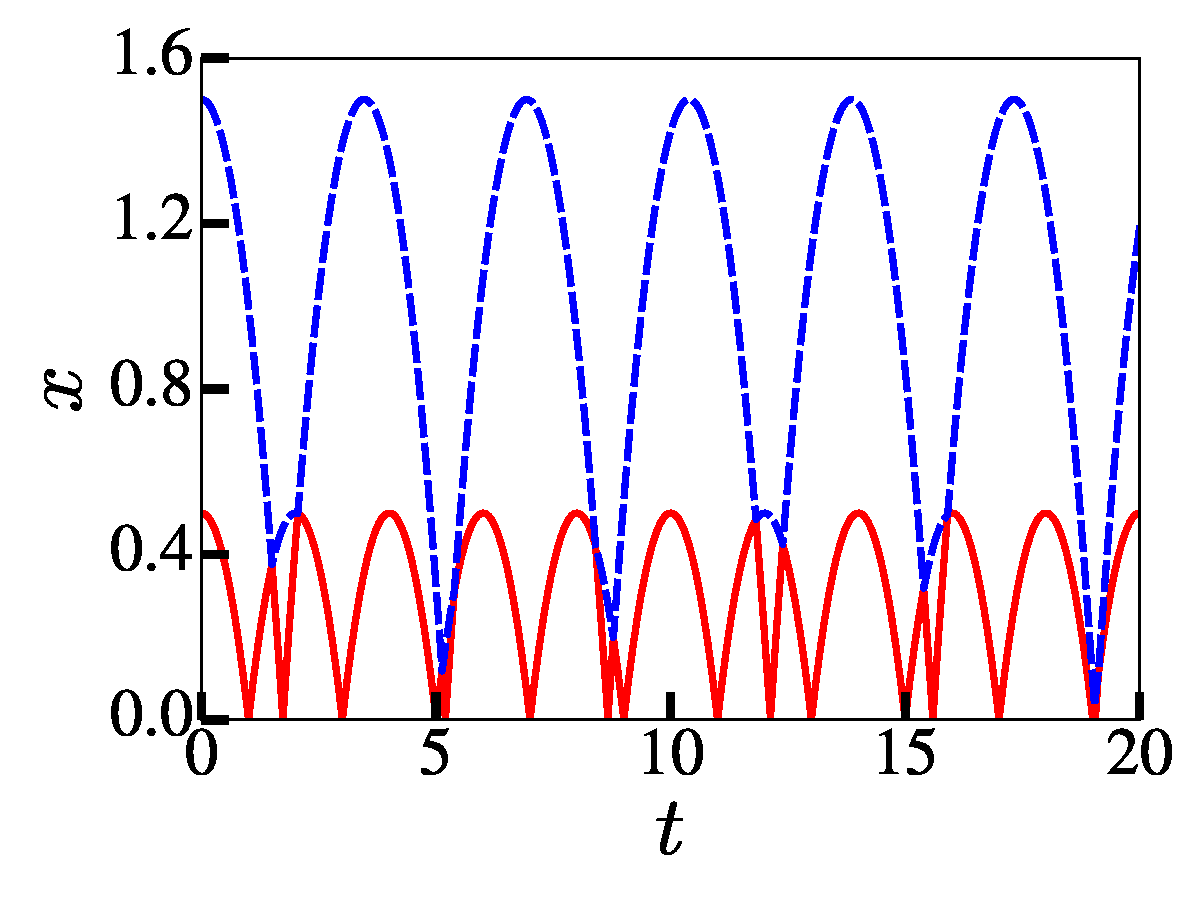
\includegraphics[width=0.8\linewidth]{r1_0_traj}
  \caption{Trajectories for two balls}
  \label{fig:1-traj}
\end{figure}


% TODO: Poincare section
\begin{figure}
  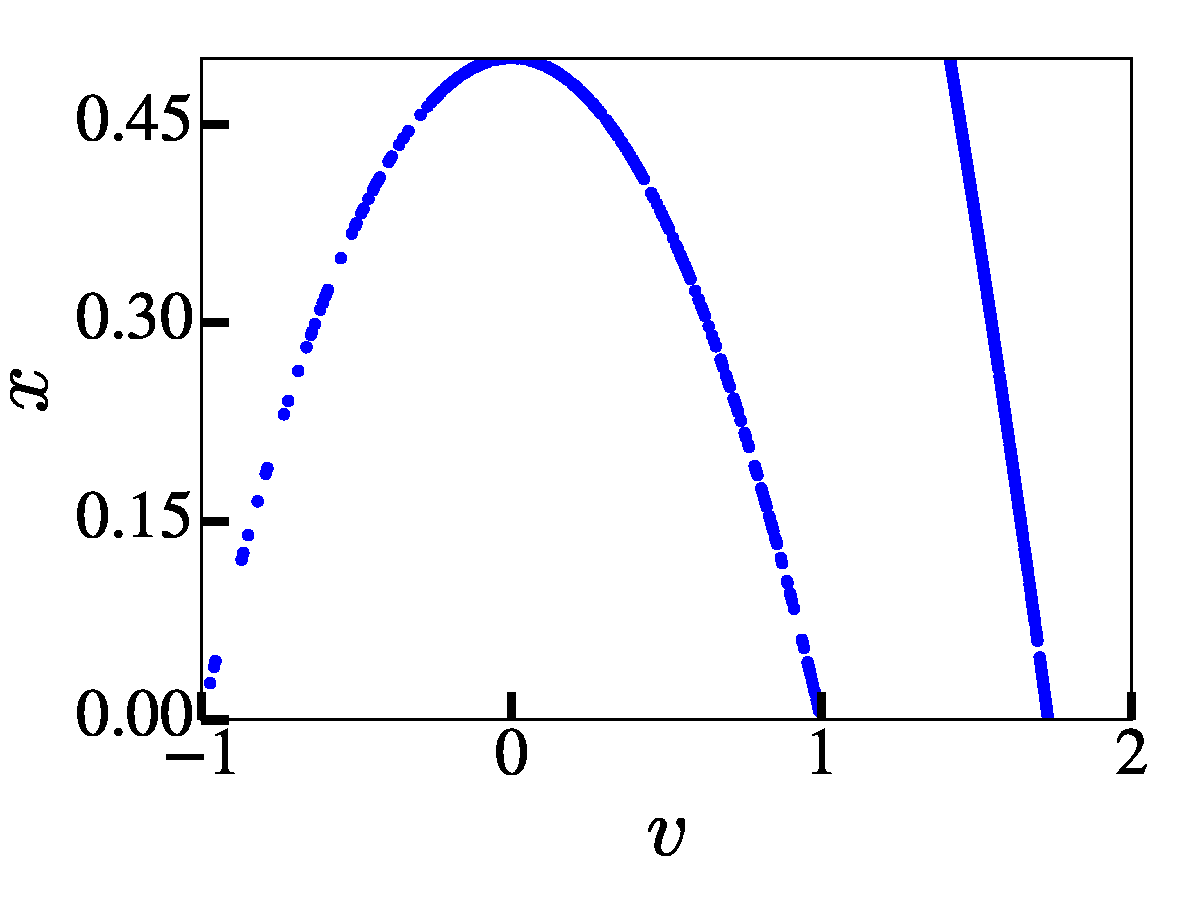
\includegraphics[width=0.8\linewidth]{r1_0_poincare}
  \caption{Poincare section for ball 2}
  \label{fig:1-poincare}
\end{figure}


% TODO: Autocorrelation function
\begin{figure}
  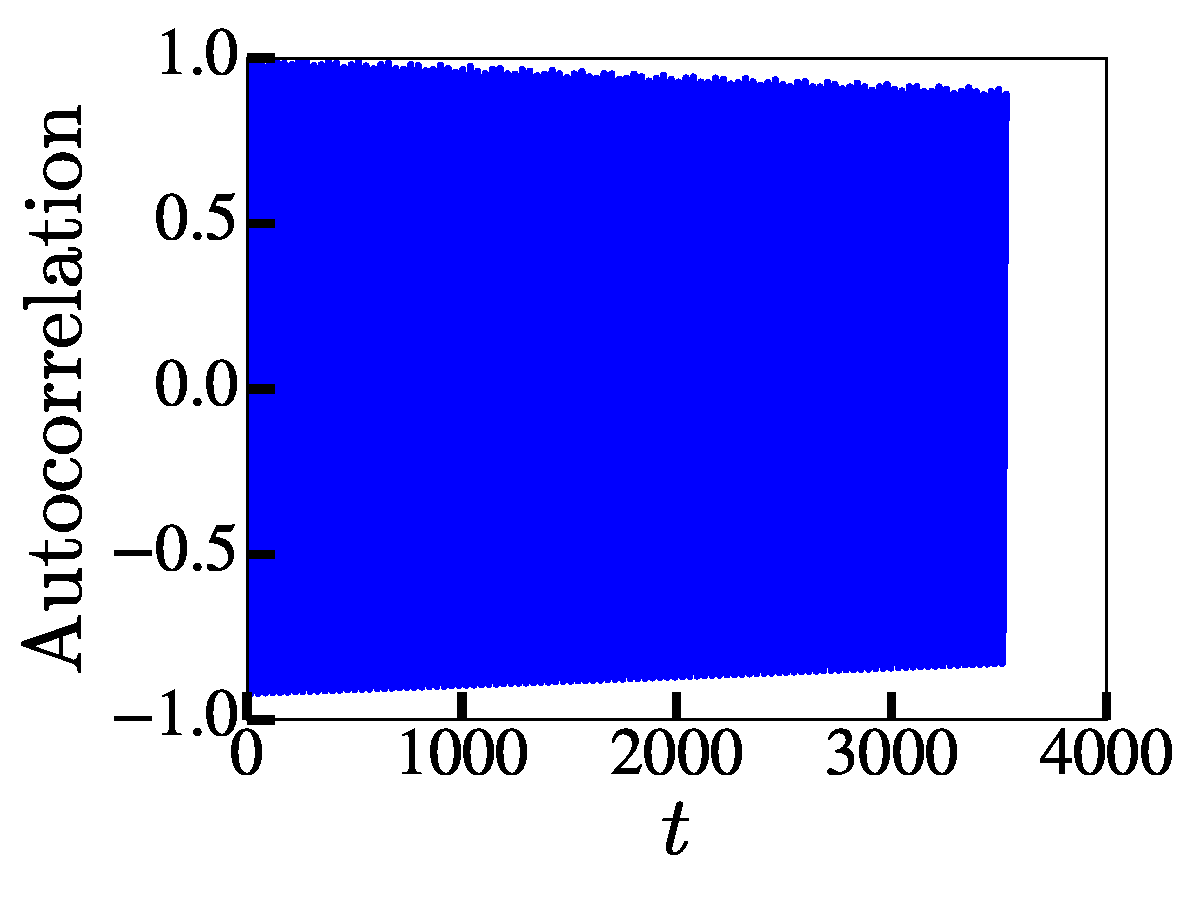
\includegraphics[width=0.8\linewidth]{r1_0_acorr}
  \caption{Autocorrelation for ball 2}
  \label{fig:1-acorr}
\end{figure}





%%%%%%%%%%%%%%%%%%%%%%%%%%% m2 = 9 m1 %%%%%%%%%%%%%%%%%%%%%%%%%%%%%%
\subsection{$m2 = 9 m1$}\label{sec:r9}
% TODO: Plots of x1 and x2 vs t for m2 = 9*m1, given initial conditions
\begin{figure}
  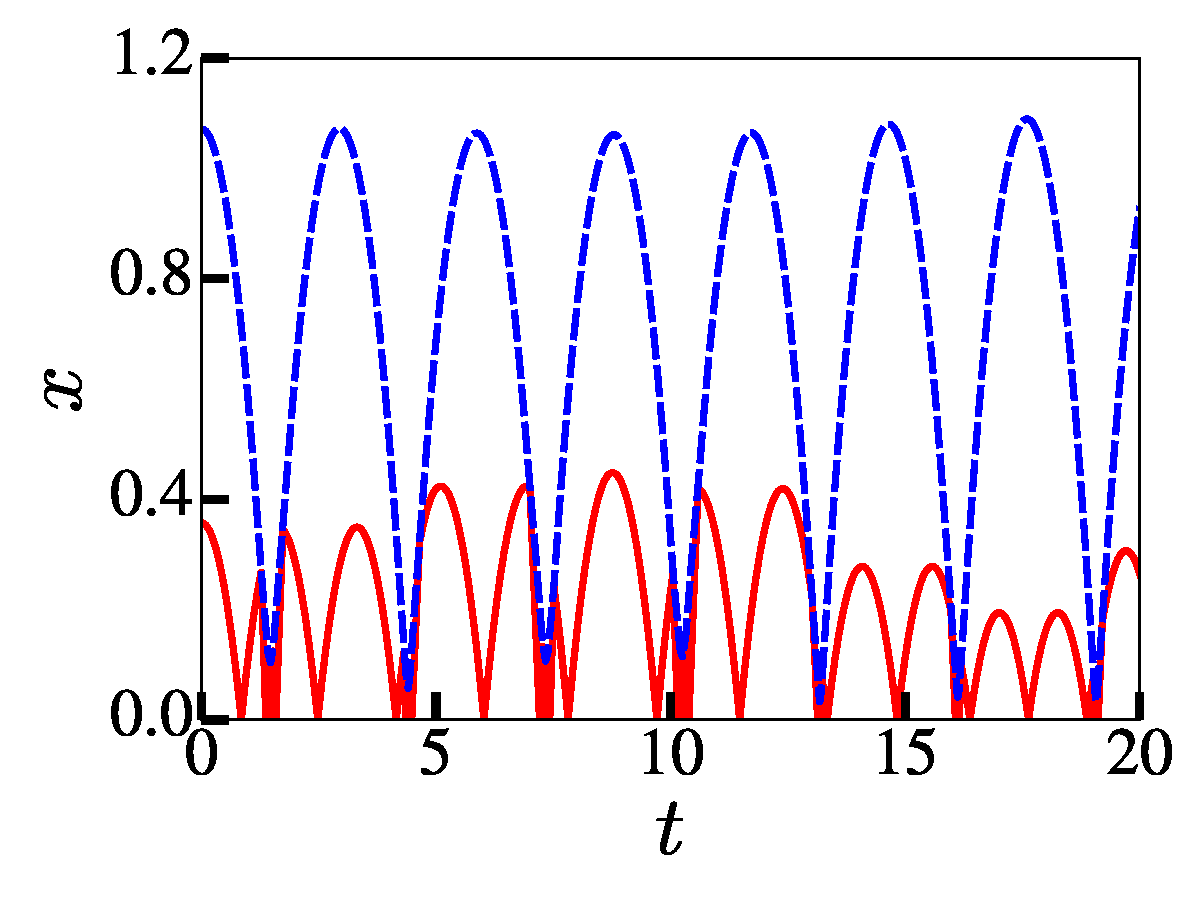
\includegraphics[width=0.8\linewidth]{r0_1_traj}
  \caption{Trajectories for two balls. The blue dashed line indicates the top
  ball, and the red line indicates the bottom ball.}
  \label{fig:9-traj}
\end{figure}


\begin{figure}
  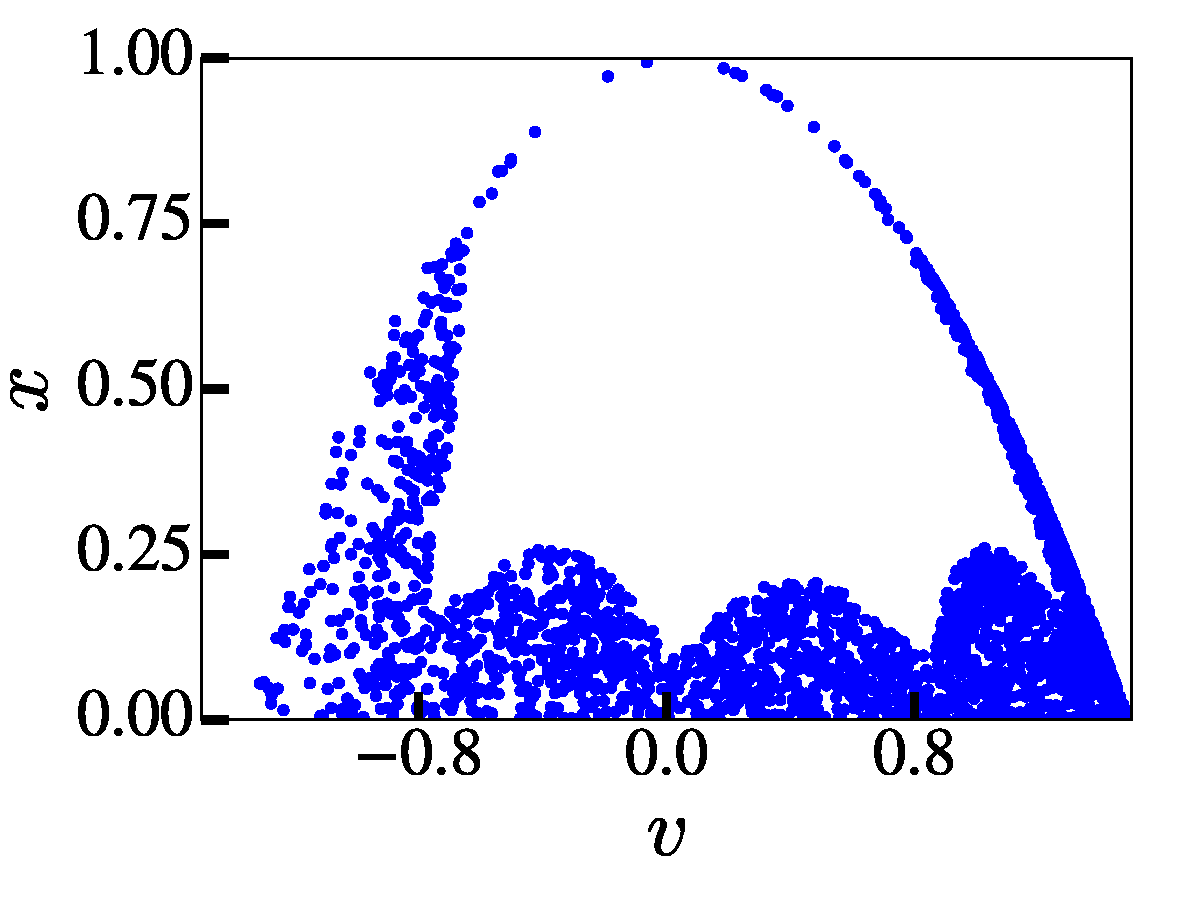
\includegraphics[width=0.8\linewidth]{r0_1_poincare}
  \caption{Poincare section for ball 2}
  \label{fig:9-poincare}
\end{figure}


\begin{figure}
  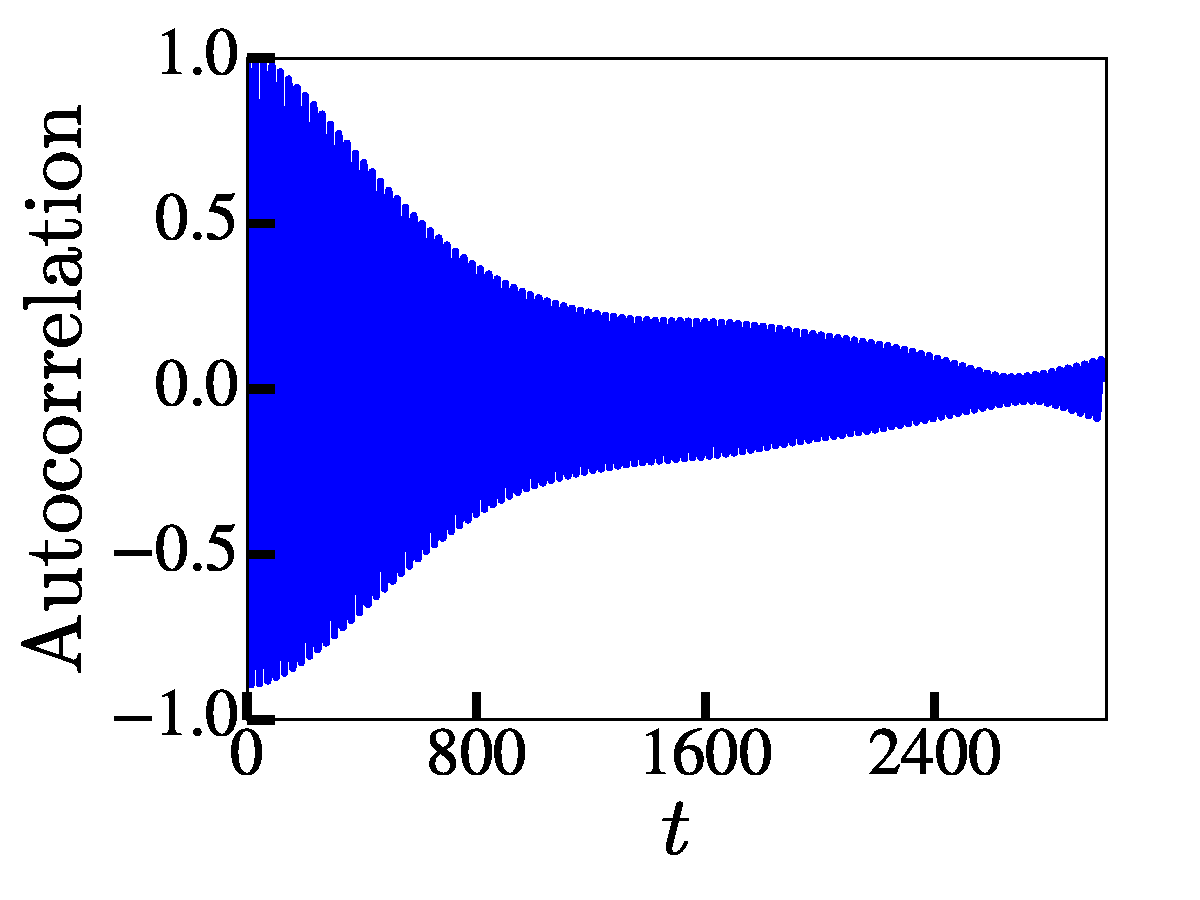
\includegraphics[width=0.8\linewidth]{r0_1_acorr}
  \caption{Autocorrelation for ball 2. T = 1500, 10\% lag}
  \label{fig:9-acorr}
\end{figure}

\subsubsection{Nonchaotic}



% TODO: Show non-chaotic Poincare section + autocorrelation function. Use Lyapunov to prove nonchaotic
\begin{figure}
  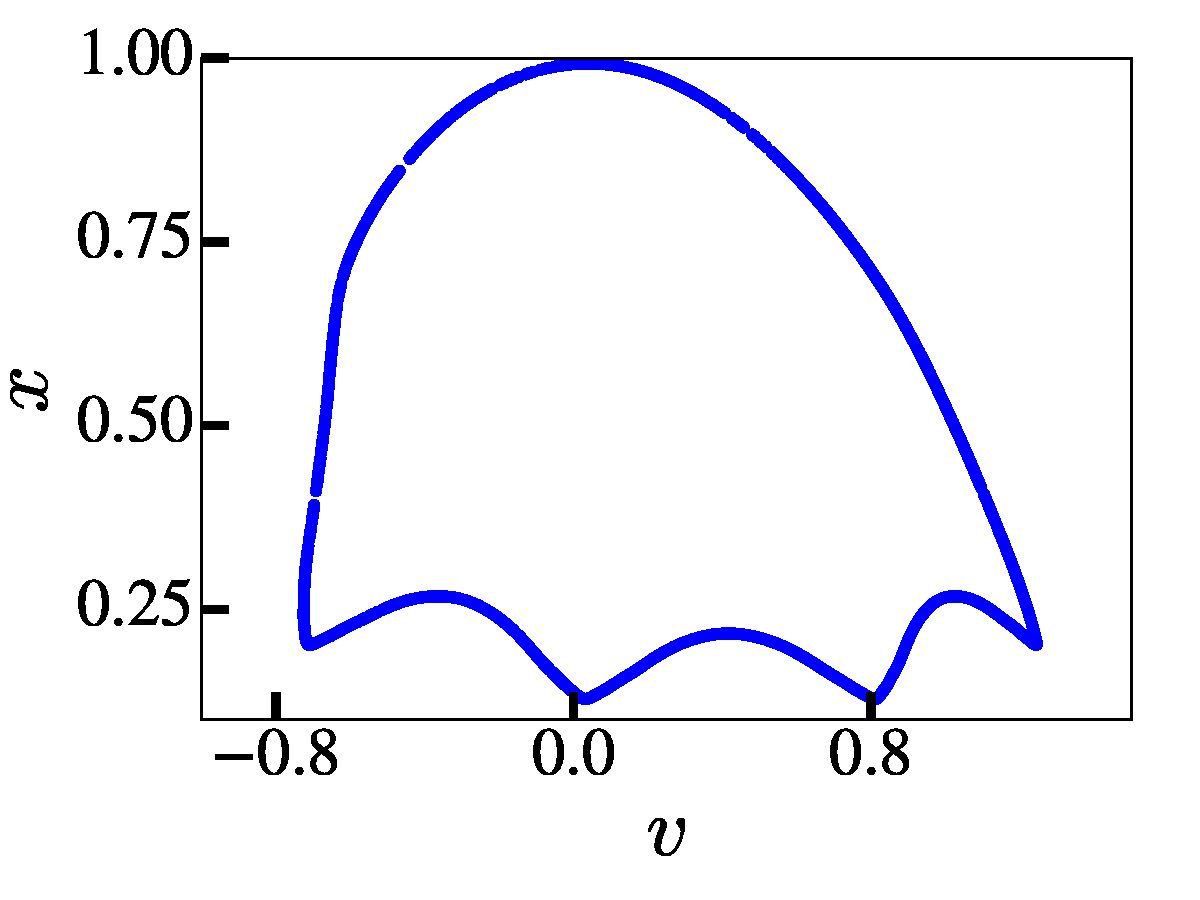
\includegraphics[width=0.8\linewidth]{nonchaotic_r0_1_poincare}
  \caption{Poincare section for ball 2. T=1500. 12 evenly spaced datapoints for
  x2 = 1.01 to 8. Darker colors indicate lower x2. v1 = 1.5, v2 = 0, x1 = 1} %TODO: When does chaotic behavior set in?
  \label{fig:0.9-traj-nonchaotic}
\end{figure}
% TODO: Comment on structure of non-chaotic Poincare section

% TODO: Calculate Lyapunov exponent for a nonchaotic system

% TODO: Comment on which are chaotic



\section{Conclusions} \label{sec:conclusion}

% TODO: Summarize project
% TODO: Highlight findings
% TODO: Discuss significance
% TODO: Future improvements



\begin{thebibliography}{1}
\bibitem{taylor}
  Taylor, J. R. (2005).
  \textit{Classical mechanics}.
  Sausalito, CA: University Science Books.

\bibitem{whelan}
Whelan, N. D., Goodings, D. A. \& Cannizzo, J. K. (1990).
Two balls in one dimension with gravity.
\textit{Phys. Rev. A}, 42, 742-754.
% TODO: Cite whelan and that other paper
\end{thebibliography}

\clearpage
\appendix
\section{Trajectory Algorithm}\label{appendix:traj}
In creating the algorithm for sampling ball trajectories at evenly-spaced times,
a few computational optimizations were made to optimize runtime.

A general overview of the algorithm is provided in Section~\ref{sec:methods}.
Each interval between events corresponds to a list element which is itself a list
of \texttt{[start\_time,~end\_time,~x\_func,~v\_func]}, where \texttt{start\_time}
and \texttt{end\_time} are the start and end times of that interval, and
\texttt{x\_func} and \texttt{v\_func} are lambda functions that return the
position and velocity of the ball at some time since the previous interval. A
list of lists is created for each ball.

This method was originally chosen to work with NumPy's \texttt{piecewise()}
function, which as the name suggests will piecewise evaluate a list of functions
over a list of input values according to a matrix of boolean values that specifies
when each function is valid for each input. However, generating this boolean matrix
was a slow task, and the boolean matrix has dimension
$sampled-times \times number of events$. %TODO: Represent this better
This matrix rapidly grows extremely large, and becomes very slow to manipulate.

Instead, a simpler solution was found by exploiting the fact that the lists of
intervals are already in sequential order. As the timesteps are iterated over,
the first element of the list of intervals is used. Once the time being sampled
is larger than the end time of that interval, the sub-list corresponding to that
element is removed from the list of intervals, and the first element in the list
of intervals becomes the next interval. This avoids usage of \texttt{piecewise()}
entirely.

A side effect of this method is that no form of array searching to find the
appropriate interval to evaluate the function over is necessary - only the first
element is ever used.


\end{document}
